\chapter{heights.h Documentation}
\ifsingle
\maketitle
\fi
\chaptermeta[2.0][2025-06-08]

\section{Introduction}\label{sec:heights-intro}
\texttt{heights.h}, together with \texttt{parabola.h}, serves as a toolbox for \texttt{curvature.h} to compute surface curvature in multiphase flow. The aim of the file is to allocate a value representing the distance to the surface for every cell. This value is named `height`, hence the name of the header file. Before diving into details, several conceptual definitions are introduced with a 1D example.

\subsection{Surface}
For each cell, if a `coherent surface' occurs within a certain distance, the cell is assigned a valid height value. Otherwise, an invalid data value `nodata' is allocated. A `coherent surface' is defined as a process where the color function (volume fraction in the VOF method) \para{c} changes from $0$ to $1$ or vice versa.

\begin{figure}[H]
  \centering
  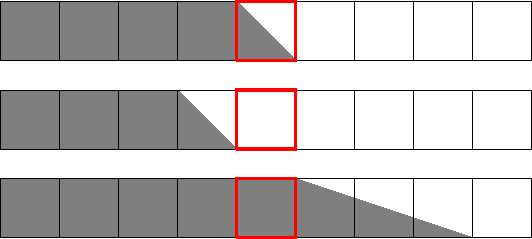
\includegraphics{./image/heights-h/surface.pdf}
  \caption{Graphical representation of a coherent surface. The cell highlighted by a red square represents the current cell. The grey color indicates volume fraction.}
  \label{fig:heights-surface}
\end{figure}
As shown in figure \ref{fig:heights-surface}, height values are valid for the current cell (highlighted by a red square) when, within a certain distance, cells fully immersed in the color function (represented by grey) and those with a $0$ value both occur. In contrast, figure \ref{fig:heights-nosurface} demonstrates cases where a `coherent surface' is not observed, so `nodata' is assigned.

\begin{figure}[H]
  \centering
  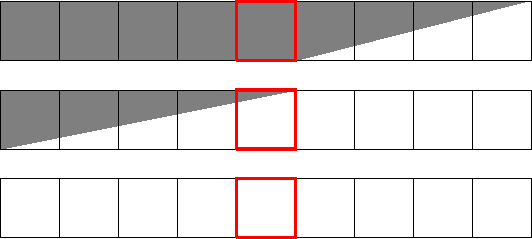
\includegraphics{./image/heights-h/nosurface.pdf}
  \caption{Graphical representation of a non-coherent surface. The cell highlighted by a red square represents the current cell. The grey color indicates volume fraction.}
  \label{fig:heights-nosurface}
\end{figure}

\subsection{Height Value and Zero-Value Point}
The height value is essentially a summary of the color function, with each cell’s value represented at its center. To obtain a specific value, the position where the value is $0$ (the zero-value point) must first be defined. Consider the condition illustrated in figure \ref{fig:heights-0position}, where the surface spans two cells with color function values of $0.6$ and $0.1$. The zero-value point is located $0.7$ units away from the last occupied cell, as indicated by the blue dashed line in figure \ref{fig:heights-0position}. The value of each cell is then calculated based on the distance between its center and the zero-value point, as shown below the figure. The positive direction points toward the inner side of the surface.

\begin{figure}[H]
    \centering
    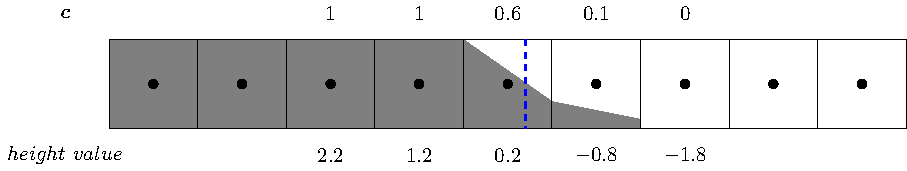
\includegraphics[width=0.65\textwidth]{./image/heights-h/0position}
    \caption{Graphical representation of the zero-value point. The blue dashed line indicates the exact position of the zero-value point. Numbers at the top show the color function of each cell, while those below display the corresponding height value at the center of each cell, marked by a black dot.}
    \label{fig:heights-0position}
\end{figure}

\subsection{Direction of Surface}
Besides the example in figure \ref{fig:heights-0position}, another possibility exists where the surface extends in the opposite direction (from right to left in this example). To distinguish these cases, the zero-value point is assigned a value of $20$ for cases shown in figure \ref{fig:heights-direction}. Typically, only cells within a $5.5$-unit distance from the zero-value point have valid height values. Thus, the range of height values is $[-5,5]$ or $[15,25]$, depending on the surface direction.

\begin{figure}
    \centering
    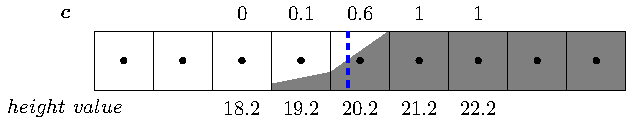
\includegraphics{./image/heights-h/direction}
    \caption{Graphical representation of the zero-value point. The blue dashed line indicates the exact position of the zero-value point. Numbers at the top show the color function of each cell, while those below display the corresponding height value at the center of each cell, marked by a black dot.}
    \label{fig:heights-direction}
\end{figure}

\section{Functions}\label{sec:heights-funcc}
\subsection{Overall Configuration}\label{sec:heights-config}
Before introducing parameters and workflows, a brief overview of the configuration of the three main functions discussed in the following sections is provided. As shown in figure \ref{fig:heights-funcconfig}, \func{heights} acts as a controller, issuing commands to \func{half\_column}, which integrates volume fractions in neighboring cells. After iterating over the eight adjacent cells (four in both positive and negative directions), the height value is assigned to the current cell. Special care is taken for tree grids, where the additional function \func{refine\_h\_x} is used to prolongate the color function.

\begin{figure}
    \centering
    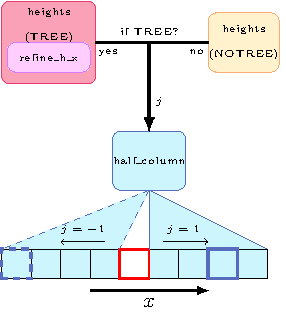
\includegraphics[width=0.5\textwidth]{./image/heights-h/heights}
    \caption{Overall configuration of the current header file. The red square highlights the current cell, and the blue square represents cells scanned by \func{half\_column}.}
    \label{fig:heights-funcconfig}
\end{figure}

\subsection{\func{height} and \func{orientation}}
\subsubsection{Worth Mentioning Details}
These two functions are `tricky' functions. As discussed in section \ref{sec:heights-intro}, to distinguish surface orientation, the final height value has two ranges: $[-5,5]$ or $[15,25]$. The \func{height} function is a reverse function that takes the height value as input, removes the orientation disguise, and returns the true distance between the current cell and the zero-value point, with an output range of $[-10,10]$. In contrast, \func{orientation} returns the surface orientation based on the height value. To save memory, these tricky functions are implemented as `inline' functions, meaning their code is substituted directly when called.

\begin{codesection}{subsubsection}{Program Workflow}
\codecomment{
  \textbf{Starting Point for \func{height}}\\
  \textbf{Input}: \para{H} (height value).\\
  The disguise value \para{HSHIFT} is $20$. By adding or removing this value, the true interfacial distance is revealed.
}
\begin{minted}{cpp}
#define HSHIFT 20.

static inline double height (double H) {
  return H > HSHIFT/2. ? H - HSHIFT : H < -HSHIFT/2. ? H + HSHIFT : H;
}
\end{minted}
\codearrow
\codecomment{
  \textbf{Starting Point for \func{orientation}}\\
  \textbf{Input}: \para{H} (height value).\\
  Returns \texttt{TRUE} or \texttt{FALSE} based on the disguise value. Two layers of ghost values are set on every boundary.
}
\begin{minted}{cpp}
static inline int orientation (double H) {
  return fabs(H) > HSHIFT/2.;
}

#define BGHOSTS 2
\end{minted}
\end{codesection}

\subsection{\func{half\_column}}
Based on the previous discussion, \func{half\_column} plays a major role in height computation by scanning neighboring cells and returning the surface status and height value. Due to its complexity, the algorithm is explained part by part.

\subsubsection{Parameters}
\begin{center}
  \begin{tabular}{|c|c|c|c|c|}
    \hline
    Name & Data type & Status & Option/Default & Representation (before/after)\\[0.5ex]
    \hline\hline
    \para{point} & Point & unchanged & compulsory & current cell position\\
    \hline
    \para{c} & scalar & unchanged & compulsory & $c$ (volume fraction)\\
    \hline
    \rowcolor{output}\para{h} & vector & \textbf{output} & compulsory & $\mathbf{h}$\\
    \hline
    \para{cs} & scalar & unchanged & compulsory & $c[2*j]$\\
    \hline
    \para{j} & int & unchanged & compulsory & $j$ (direction control)\\
    \hline
  \end{tabular}
\end{center}

\subsubsection{Purpose of the Function}\label{sec:heights-purpose}
\func{half\_column} has two purposes:
\begin{enumerate}
    \item To check whether a coherent surface (defined in section \ref{sec:heights-intro}) exists within eight adjacent cells.
    \item If a coherent surface exists, compute the corresponding height value by integrating the color function of each cell.
\end{enumerate}
There are three possible situations for the current cell: $f_c=1$, $f_c=0$, or $f_c\in(0,1)$, where $f_c$ is the color function value. For the first two cases, the threshold for a coherent surface is finding a neighbor with $f=0$ or $f=1$, respectively. For the third case (a surface cell), both directions must be iterated to find a pair of opposite (full and empty) cells on each side.

\begin{figure}
    \centering
    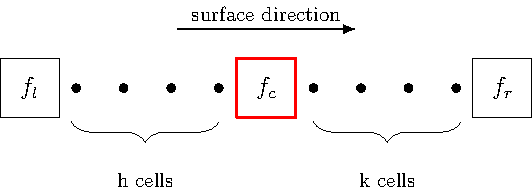
\includegraphics{./image/heights-h/possw}
    \caption{Sketch of position switching between cells. $f_c$, $f_r$, $f_l$ represent the color function values of the current cell (red square) and its right/left neighbors, respectively.}
    \label{fig:heights-possw}
\end{figure}

Once a coherent surface is found, the remaining task is to calculate the height value. The key is understanding position switching between cells. As shown in figure \ref{fig:heights-possw}, where $f_c$, $f_r$, $f_l$ represent the color function values of the current cell and its neighbors, following the surface direction (defined as a vector pointing from the inner to the outer side of the surface, e.g., figure \ref{fig:heights-0position}), the relationship between these values is:
\begin{align}
    f_c - (k+1) = f_r\\
    f_c + (h+1) = f_l
\end{align}
Among all cells, the easiest height value to compute is that of the final full cell close to the surface (hereinafter called the final cell). Figure \ref{fig:heights-hvcomp} revisits the example from figure \ref{fig:heights-0position}, highlighting the final cell and surface direction. Based on section \ref{sec:heights-intro}, the height value of the final cell is computed by integrating the color function along the surface direction until the first empty cell (cell $E$):
\begin{equation}
    h_B = h_B + h_C + h_D + h_E - 0.5 = 1 + 0.6 + 0.1 + 0 - 0.5 = 1.2
\end{equation}
The four terms on the right-hand side represent the color function values of cells $B$, $C$, $D$, and $E$. The $-0.5$ accounts for the fact that the height value is determined from the cell’s center, not its left boundary. Using position switching, the height value of every cell can be obtained. For example, the height value of cell $F$ is $h_F = h_B - 4 = -2.8$, and that of cell $A$ is $h_A = h_B + 1 = 2.2$.

\begin{figure}
    \centering
    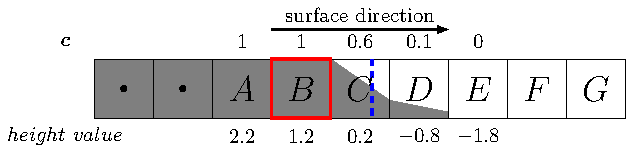
\includegraphics{./image/heights-h/hvcomp}
    \caption{Same example as in figure \ref{fig:heights-0position} with two example stencils $A$, $B$. The red square highlights the final full cell next to the surface.}
    \label{fig:heights-hvcomp}
\end{figure}

\subsubsection{Configuration of the Function}
Figure \ref{fig:heights-column} details the configuration of \func{half\_column}, which consists of three layers. As shown in figure \ref{fig:heights-funcconfig} and section \ref{sec:heights-funcc}, \func{half\_column} is called twice: first for the negative direction ($j=-1$), then for the positive direction ($j=1$). Except for the second layer (`iteration'), the other two layers are adjusted based on the direction.

Parameter \para{S} records the process status: if a surface is found, the height computation is complete (\para{S} = $-1$); if one end is found, \para{S} = $1$ or $0$; if no end is found, \para{S} $\in (0,1)$. Since \para{S} is defined within \func{half\_column} and cleared when the function ends, a method is needed to preserve results from the negative direction. Basilisk achieves this by encoding the status and height result \para{H} into \para{h[]} and decoding it at the start of the second cycle ($j=1$).

In the overall process, decoding (if needed) occurs with initial settings in the first layer. Height values are calculated and stored as \para{H} in the second layer by checking neighboring cells, with \para{S} updated accordingly. The output \para{h[]} is processed in the final layer, either encoded or directly output, depending on the direction. Detailed explanations follow.

\subsubsection{First Layer}
The initial status \para{S} is derived from the volume fraction of the current cell (highlighted by a red square) and can be $0$, $1$, or $f$ (empty, full, or surface cell). In the second cycle ($j=1$), an additional decoding step restores the status and height from the previous cycle into \para{stats.s} and \para{stats.h}. Four decoding scenarios are possible:
\begin{enumerate}
    \item $\para{h[]}=300$, $(\para{stat.s},\para{stat.h})=(-1,\text{nodata})$: Non-surface cells ($\para{c[]}=1$ or $0$) that fail to find a coherent surface, or surface cells that fail to find an empty/full cell in the first cycle.
    \item $90\leq\para{h[]}<190$, $(\para{stat.s},\para{stat.h})=(0,\para{h[]}-100)$: Surface cells that find an empty cell in the first cycle.
    \item $190\leq\para{h[]}$, $(\para{stat.s},\para{stat.h})=(-1,\para{h[]}-200)$: Surface cells that find a full cell in the first cycle.
    \item $-10\leq\para{h[]}<90$, $(\para{stat.s},\para{stat.h})=(-1,\para{h[]})$: Empty/full cells that find a coherent surface in the first cycle.
\end{enumerate}
For scenarios 2 and 3, \para{S} and \para{H} are set to \para{stats.s} and \para{stats.h} to continue searching for the other end. Otherwise, \para{S} and \para{H} retain their initial values.

\subsubsection{Second Layer}
As shown in figure \ref{fig:heights-column}, there are five categories of scenarios leading to four types of results, stemming from three types of \para{S} rather than the current cell’s volume fraction:
\begin{itemize}
    \item[A] $0<\para{S}=f<1$: Find an empty/full cell, \para{S} switches to $0$/$1$, resulting in condition \Romannum{1}/\Romannum{2}. One end of a coherent surface is found.
    \item[B] $\para{S}=1$: Find an empty cell, indicating a coherent surface. \para{S} switches to $-1$, completing the iteration (condition \Romannum{3}).
    \item[C] $\para{S}=0$: Find a full cell, indicating a coherent surface. \para{S} switches to $-1$, completing the iteration (condition \Romannum{3}).
    \item[D] $\para{S}=1$ or $\para{S}=0$: Scan a surface cell and return to one with the same status as \para{S}. Since the program scans only four neighboring cells, this suggests failure to find a coherent surface in this direction, addressing cases like figure \ref{fig:heights-Dtarget}. This leads to condition \Romannum{4}, with \para{S} unchanged.
    \item[Others]: All other cases fail to find a coherent surface or at least one end, leaving \para{S} unchanged and leading to condition \Romannum{4}.
\end{itemize}

\begin{figure}
    \centering
    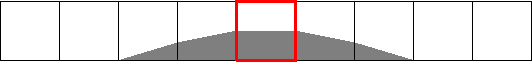
\includegraphics{./image/heights-h/Dtarget}
    \caption{The situation that the second layer occasion D aims to tackle.}
    \label{fig:heights-Dtarget}
\end{figure}

Height value accumulation occurs in this layer, implicitly shown in figure \ref{fig:heights-column}. Following the protocol in section \ref{sec:heights-purpose}, the height value is computed and adjusted by adding \para{HSHIFT} = $20$ if the surface direction opposes the coordinate, as discussed in section \ref{sec:heights-config}.

\subsubsection{Third Layer}\label{sec:heights-thirdl}
For the negative direction ($j=-1$), the output status and height value are encoded into \para{h[]} in this layer. The four conditions from the second layer are grouped into three categories:
\begin{itemize}
    \item[A] Condition \Romannum{4}, encoded as $\para{h[]}=300$: Cases failing to find a coherent surface, marked as `inconsistent'.
    \item[B] Condition \Romannum{3}, not encoded, $\para{h[]}=\para{H}$: Cases successfully finding a coherent surface.
    \item[C] Conditions \Romannum{1} and \Romannum{2}, encoded as \Romannum{1}: $\para{h[]}=\para{H}+100$, \Romannum{2}: $\para{h[]}=\para{H}+200$: Surface cells finding an empty/full cell as one end of a coherent surface.
\end{itemize}

For the positive direction ($j=1$), the third layer serves as the final output. Before assigning \para{h[]}, two scenarios update the data as $(\para{stats.s},\para{stats.h})=(\para{S},\para{H})$:
\begin{enumerate}
    \item Condition \Romannum{5}: Surface cell as the current cell, finding one end in the first cycle.
    \item Condition \Romannum{3}: Coherent surface found in the second cycle, with the second cycle’s height value less than the first cycle’s, i.e., $\para{H}<\para{stats.h}$.
\end{enumerate}
The second scenario ensures that when a cell has two valid height values, the smaller one is used. Since \para{nodata} is a large integer in Basilisk, this also covers cases failing in the first cycle but succeeding in the second.

The final height value \para{h[]} is assigned based on $(\para{stats.s},\para{stats.h})$, as shown in figure \ref{fig:heights-column}.

\begin{figure}
    \centering
    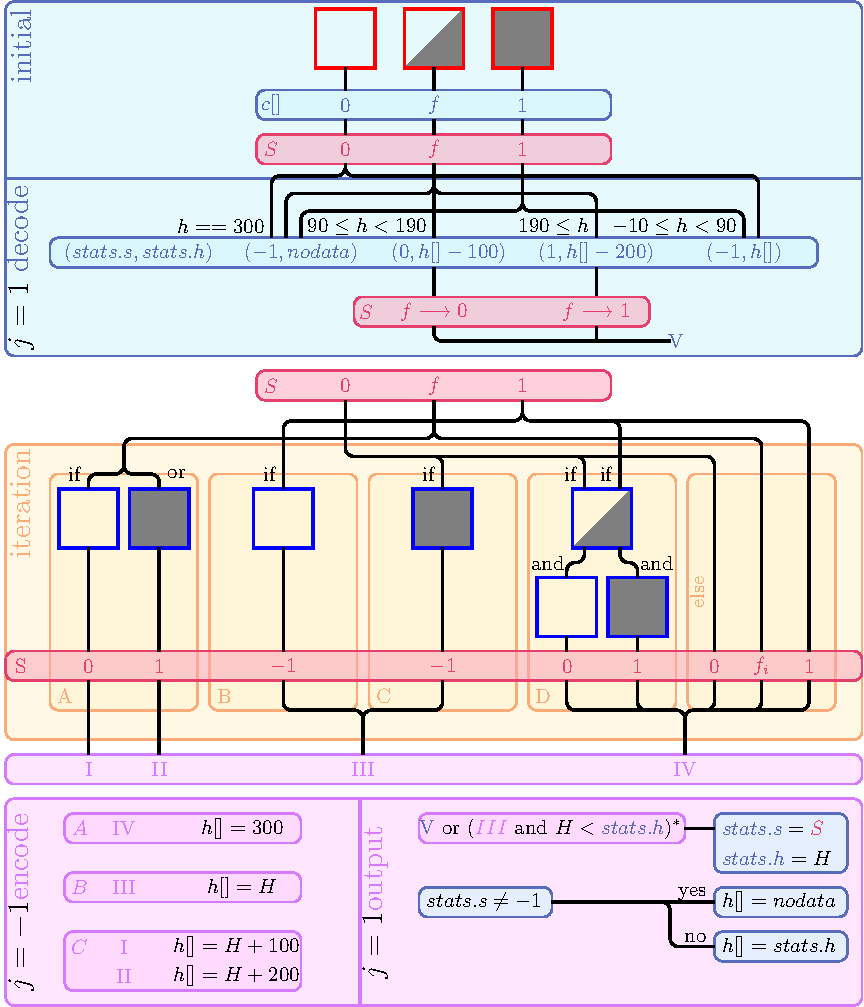
\includegraphics{./image/heights-h/column}
    \caption{Detailed description of \func{half\_column}. For simplicity, some tricky treatments are hidden. For instance, the judgment in the third layer highlighted by $\ast$ compares surface distance rather than direct values of $H$ and $stats.h$. Thus, the actual judgment is $fabs(height(H))<fabs(height(stats.h))$.}
    \label{fig:heights-column}
\end{figure}

\begin{codesection}{subsubsection}{Program Workflow}
\codecomment{
  \textbf{First Layer: Initial Setup}\\
  \textbf{Input}: \para{point}, \para{c}, \para{h}, \para{cs}, \para{j}.\\
  Initialize \para{S} = $f$, \para{H} = $f$, where \para{ci} and \para{a} are used in the second layer. Iterates over each dimension to compute \para{h.x}, \para{h.y}, \para{h.z}.
}
\begin{minted}{cpp}
static void half_column (Point point, scalar c, vector h, vector cs, int j)
{
  const int complete = -1;
  foreach_dimension() {
    double S = c[], H = S, ci, a;
\end{minted}
\codearrow
\codecomment{
  \textbf{First Layer: Decode (Part 1)}\\
  If the condition is inconsistent (condition \Romannum{4}), set \para{state.h} = $-1$ and begin a new iteration.
}
\begin{minted}{cpp}
    typedef struct { int s; double h; } HState;
    HState state = {0, 0};
    if (j == 1) {
      if (h.x[] == 300.)
        state.s = complete, state.h = nodata;
\end{minted}
\codearrow
\codecomment{
  \textbf{First Layer: Decode (Part 2)}\\
  Decode cases other than condition \Romannum{4}. Since \para{s} is an integer, only cases with $\para{h[]}\geq 90$ (conditions \Romannum{2} and \Romannum{3}) yield non-zero \para{s}, restoring previous status as $(\para{S},\para{H})=(\para{state.s},\para{state.h})$. Otherwise (condition \Romannum{3}), the iteration uses the original initial values.
}
\begin{minted}{cpp}
      else {
        int s = (h.x[] + HSHIFT/2.)/100.;
        state.h = h.x[] - 100.*s;
        state.s = s - 1;
      }
      if (state.s != complete)
        S = state.s, H = state.h;
    }
\end{minted}
\codearrow
\codecomment{
  \textbf{Second Layer: Iteration (Part A)}\\
  Scan four neighboring cells. If $1>\para{S}>0$ and an empty or full cell is found ($\para{ci}=0$ or $\para{ci}=1$), update \para{S} and modify \para{H} based on its position relative to the zero-value point.
}
\begin{minted}{cpp}
    for (int i = 1; i <= 4; i++) {
      ci = i <= 2 ? c[i*j] : cs.x[(i - 2)*j];
      H += ci;
      if (S > 0. && S < 1.) {
        S = ci;
        if (ci <= 0. || ci >= 1.) {
          H -= i*ci;
          break;
        }
      }
\end{minted}
\codearrow
\codecomment{
  \textbf{Second Layer: Iteration (Parts B and C)}\\
  \textbf{Part B}: For full current cells finding an empty cell, stop iteration, set \para{S} to complete, and compute height as discussed.\\
  \textbf{Part C}: For empty current cells finding a full cell.
}
\begin{minted}{cpp}
      else if (S >= 1. && ci <= 0.) {
        H = (H - 0.5)*j + (j == -1)*HSHIFT;
        S = complete;
        break;
      }
      else if (S <= 0. && ci >= 1.) {
        H = (i + 0.5 - H)*j + (j == 1)*HSHIFT;
        S = complete;
        break;
      }
\end{minted}
\codearrow
\codecomment{
  \textbf{Second Layer: Iteration (Part D)}\\
  If a surface cell is scanned but no coherent surface is found, stop the iteration.
}
\begin{minted}{cpp}
      else if (S == ci && modf(H, &a))
        break;
    }
\end{minted}
\codearrow
\codecomment{
  \textbf{Third Layer: Encoding (Part A)}\\
  Inconsistent surfaces (condition \Romannum{4}) are encoded as $\para{h[]}=300$.
}
\begin{minted}{cpp}
    if (j == -1) {
      if (S != complete && ((c[] <= 0. || c[] >= 1.) || (S > 0. && S < 1.)))
        h.x[] = 300.; // inconsistent
\end{minted}
\codearrow
\codecomment{
  \textbf{Third Layer: Encoding (Part B)}\\
  Complete cases (condition \Romannum{3}) assign \para{h[]} directly as \para{H}.
}
\begin{minted}{cpp}
      else if (S == complete)
        h.x[] = H;
\end{minted}
\codearrow
\codecomment{
  \textbf{Third Layer: Encoding (Part C)}\\
  Partial heights (conditions \Romannum{1} and \Romannum{2}) are encoded based on whether an empty or full cell was found.
}
\begin{minted}{cpp}
      else
        h.x[] = H + 100.*(1. + (S >= 1.));
    }
\end{minted}
\codearrow
\codecomment{
  \textbf{Third Layer: Output (Part D)}\\
  For certain cases, update \para{state.s} and \para{state.h}. See section \ref{sec:heights-thirdl} for details.
}
\begin{minted}{cpp}
    else { // j = 1
      if (state.s != complete ||
          (S == complete && fabs(height(H)) < fabs(height(state.h))))
        state.s = S, state.h = H;
\end{minted}
\codearrow
\codecomment{
  \textbf{Third Layer: Output (Part E)}\\
  Assign \para{h[]} based on \para{state.s} and \para{state.h}.
}
\begin{minted}{cpp}
      if (state.s != complete)
        h.x[] = nodata;
      else
        h.x[] = (state.h > 1e10 ? nodata : state.h);
    }
  }
}
\end{minted}
\end{codesection}

\subsection{\func{column\_propagation}}
The \func{column\_propagation} function supplements \func{half\_column} by assigning height values to cells within $5.5R$ of the zero-value point that received `nodata' from \func{half\_column}. For example, cell $G$ in figure \ref{fig:heights-hvcomp} is valid and should have a height value of $-3.8$, but it receives `nodata' due to failing to find a coherent surface in its four neighbors. \func{column\_propagation} addresses this issue.

\subsubsection{Parameters}
\begin{center}
  \begin{tabular}{|c|c|c|c|c|}
    \hline
    Name & Data type & Status & Option/Default & Representation (before/after)\\[0.5ex]
    \hline\hline
    \rowcolor{output}\para{h} & vector & \textbf{updated} & compulsory & $\mathbf{h}$\\
    \hline
  \end{tabular}
\end{center}

\subsubsection{Worth Mentioning Details}
Similar to \func{half\_column}, this function iterates two neighbors in both directions and updates the height value based on the spatial relation with the smallest height cell.

\begin{codesection}{subsubsection}{Program Workflow}
\codecomment{
  \textbf{Propagation}\\
  \textbf{Input}: \para{h} = $\mathbf{h}$.\\
  Search four neighbors for valid height values, then update the current cell’s value. The inline function \func{height} is called to reveal the true distance to the zero-value point.
}
\begin{minted}{cpp}
static void column_propagation (vector h)
{
  foreach (serial) // not compatible with OpenMP
    for (int i = -2; i <= 2; i++)
      foreach_dimension()
        if (fabs(height(h.x[i])) <= 3.5 &&
            fabs(height(h.x[i]) + i) < fabs(height(h.x[])))
          h.x[] = h.x[i] + i;
}
\end{minted}
\end{codesection}

\subsection{\func{heights} for Non-Tree Grid}
As discussed in section \ref{sec:heights-config}, \func{heights} controls \func{half\_column} and \func{column\_propagation} to assign height values to valid cells. The non-tree grid version is presented first, sharing the same structure as the tree grid version.

\subsubsection{Parameters}
\begin{center}
  \begin{tabular}{|c|c|c|c|c|}
    \hline
    Name & Data type & Status & Option/Default & Representation (before/after)\\[0.5ex]
    \hline\hline
    \para{c} & scalar & unchanged & compulsory & color function $c$\\
    \hline
    \rowcolor{output}\para{h} & vector & \textbf{updated} & compulsory & $\mathbf{h}$\\
    \hline
  \end{tabular}
\end{center}

\subsubsection{Worth Mentioning Details}
Since the default boundary settings provide only two cells, an additional vector \para{s} is created to support iteration over four cells in both directions. The value stored at position $[x_0,y_0]$ for \para{s} is:
\begin{equation}\label{equ:heights-translation}
    s.x[x_0,y_0] = c[x_0+2j,y_0]
\end{equation}
where \para{j} indicates the direction (see figure \ref{fig:heights-funcconfig}). Each component of \para{s} represents a value translation in the corresponding direction.

\begin{codesection}{subsubsection}{Program Workflow}
\codecomment{
  \textbf{Starting Point}\\
  \textbf{Input}: \para{c} = $c$, \para{h} = $\mathbf{h}$.\\
  \textbf{Boundary Settings}: Ensure \para{s} has the same boundary settings as \para{c}.\\
  \textbf{Direction Iteration}: \para{j} represents the current direction, with $j = -1$ (resp. $1$) indicating negative (resp. positive) direction.\\
  \textbf{Value Assignment for \para{s}}: Implement equation \ref{equ:heights-translation}.
}
\begin{minted}{cpp}
#if !TREE
trace
void heights (scalar c, vector h)
{
  vector s[];
  foreach_dimension()
    for (int i = 0; i < nboundary; i++)
      s.x.boundary[i] = c.boundary[i];
  for (int j = -1; j <= 1; j += 2) {
    foreach()
      foreach_dimension()
        s.x[] = c[2*j];
\end{minted}
\codearrow
\codecomment{
  \textbf{Height Value Assignment}\\
  \textbf{Call \func{half\_column}}: Assign height values for each cell in every direction.\\
  \textbf{Call \func{column\_propagation}}: Propagate height values to ensure cells within $5.5R$ have valid height values.
}
\begin{minted}{cpp}
    foreach (overflow)
      half_column (point, c, h, s, j);
  }
  column_propagation (h);
}
\end{minted}
\end{codesection}

\printbibliography